\subsubsection{Introduction}

This section aims to add batch normalization to the neural network designed in
Part A. The effect on the neural network should be investigated in order to
determine if it increases the performance of the network.

\subsubsection{Rational}

Batch normalization works to alleviate the effects of covariate shift within a
CNN. Batch normalization allows for the use of higher training rates, and also
the use of less dropout within the network, due to the regularization effects it
has.

\subsubsection{Design}

Batch normalization was originally proposed as a layer to be placed before the
activation function, however, it has been noted that performance increases can
be found by placing the layer after the activation function. As the base model
is defined with the activation functions within the layer definitions, the
normalization layers will be placed after the activation functions.

\begin{figure}[H]
	\centering
	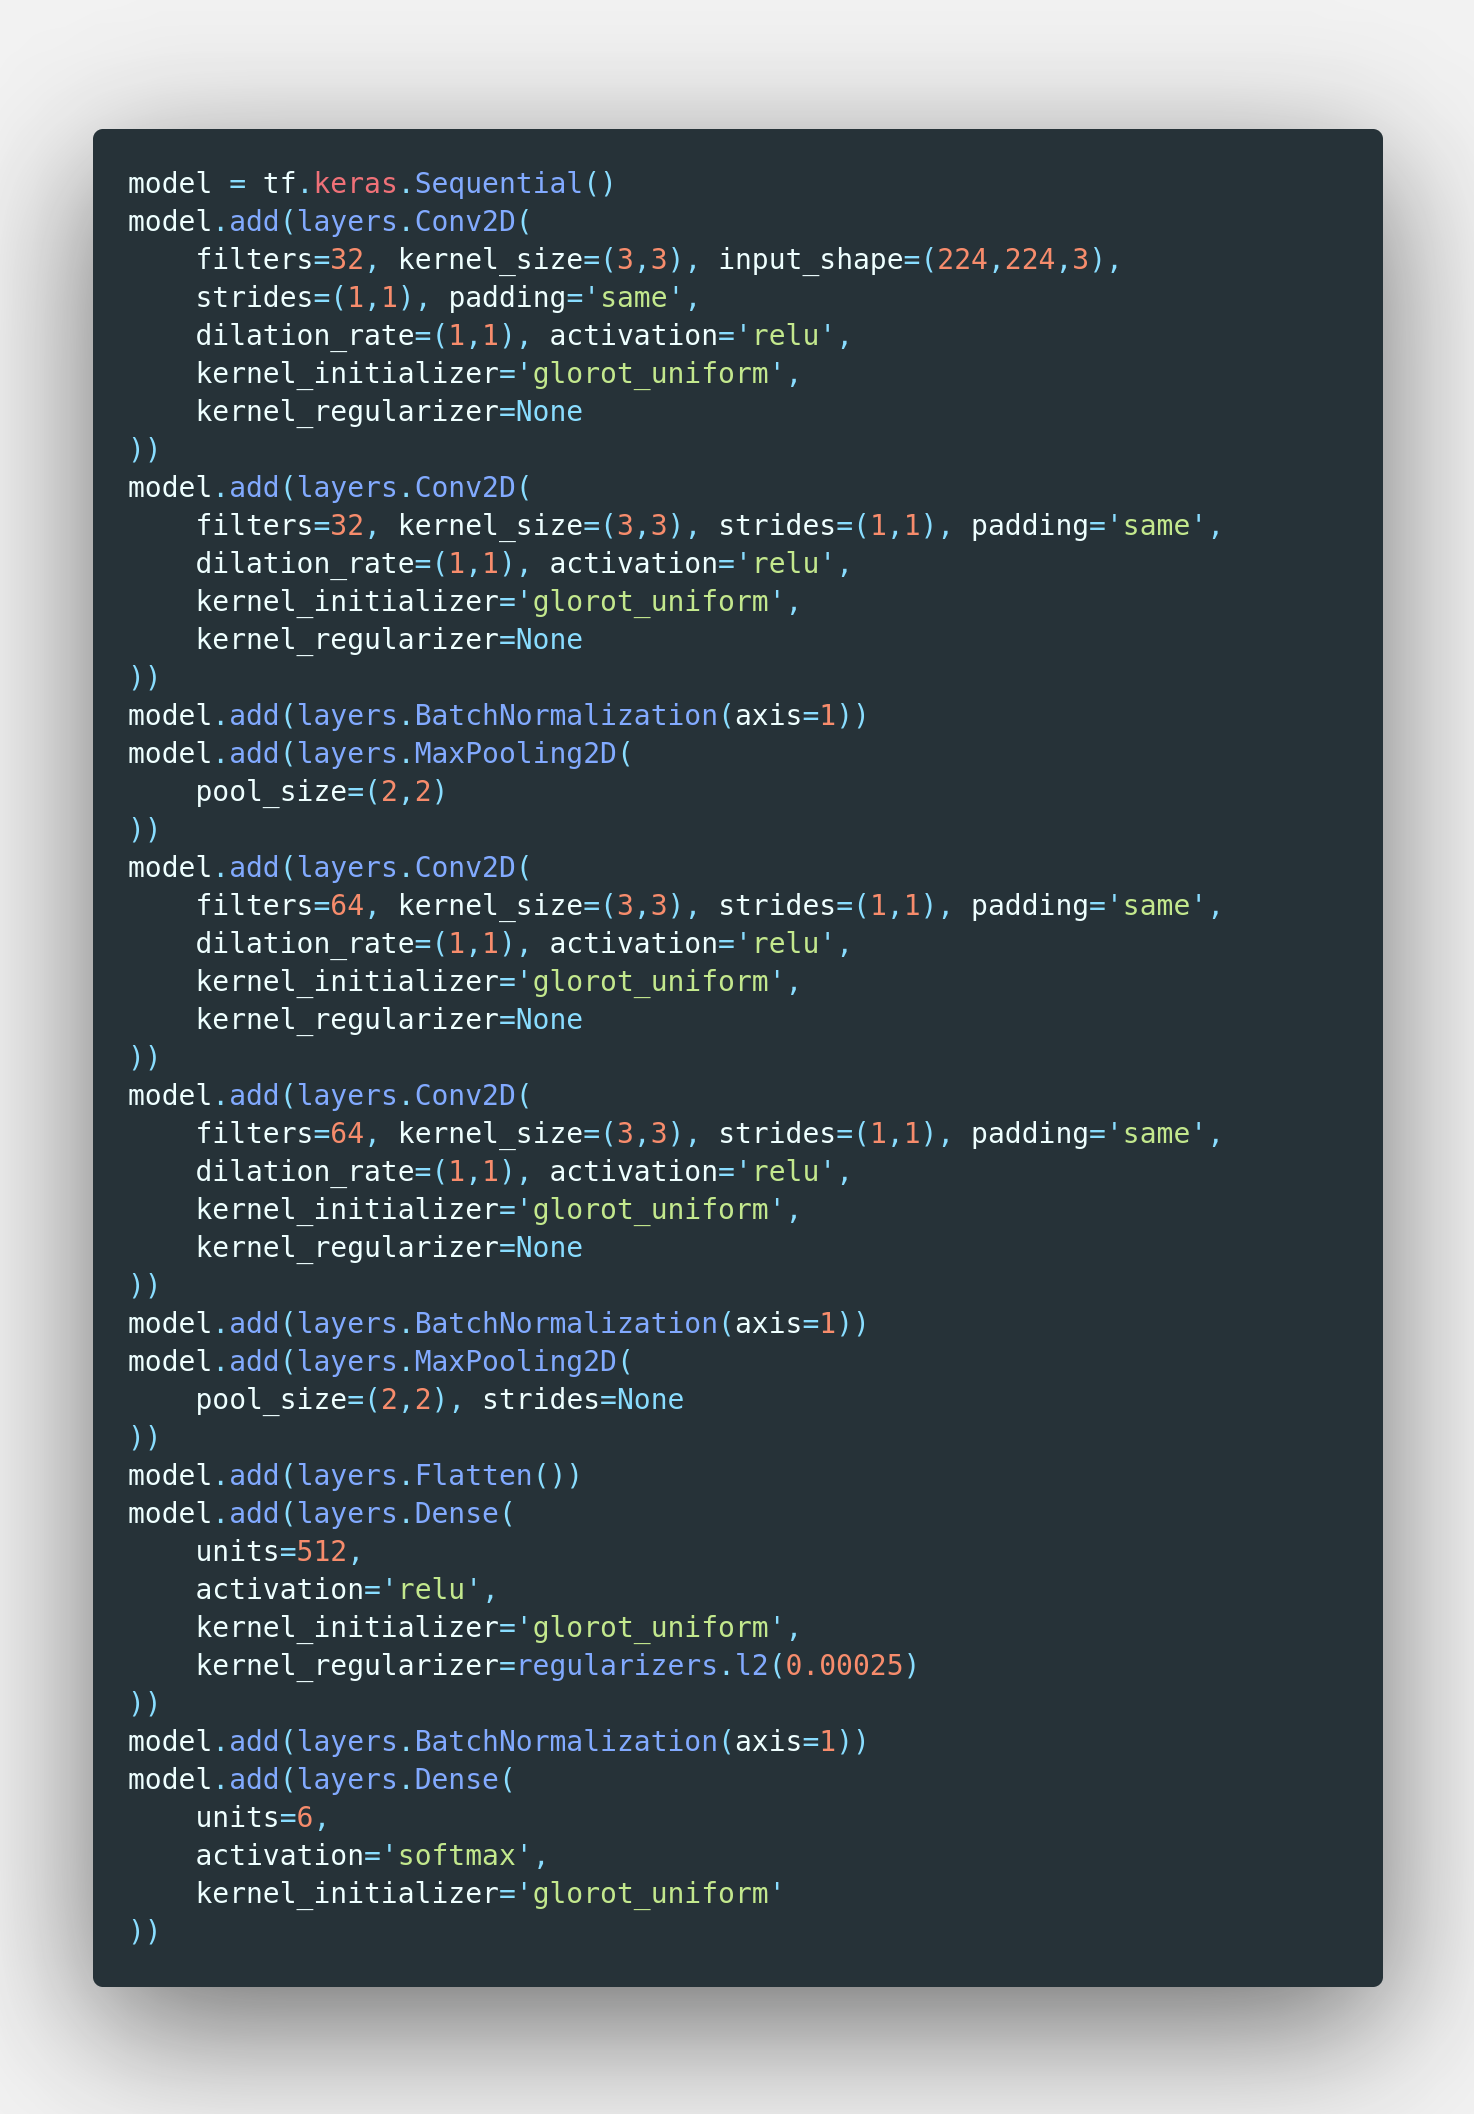
\includegraphics[width=0.8\textwidth]{images/Code/batchnorm}
	\caption{Batch Normalization Model}
	\label{fig:images-Code-batchnorm}
\end{figure}

\subsubsection{Testing}

As previously mentioned, three batch normalization layers were added to the
model. The hyperparameter being tested is the momentum, which, by default is set
to 0.99. The value of 0.5 and 0.0 were also tested, as outlined below.

\begin{table}[H]
	\centering
	\caption{Batch Normalisation Hyperparameter Tuning}
	\label{tab:bnhyp}
	\begin{tabular}{|c|c|}
	\hline
	Momentum & Validation Accuracy \\
	\hline
	0.99 & 78.83 \\
	0.5  & 78.50 \\
	0.0  & 74.33 \\
	\hline
	\end{tabular}
\end{table}

The value of 0.0 for momentum was proposed in the original paper in which batch
normalisation was introduced, however, the default value of 0.99 is shown to
have the best accuracy. As such this is the value which will be tested.

Again, the number of epochs was increased to 30, however, the early stopping
patience value left at 5, as any higher and the model would train for all 30
epochs, and give low accuracy.

\subsubsection{Results}

The model structure, as output via the ``model.summary'' function in keras, can
be seen below. The three batch normalisation layers can clearly be seen.

\begin{figure}[H]
	\centering
	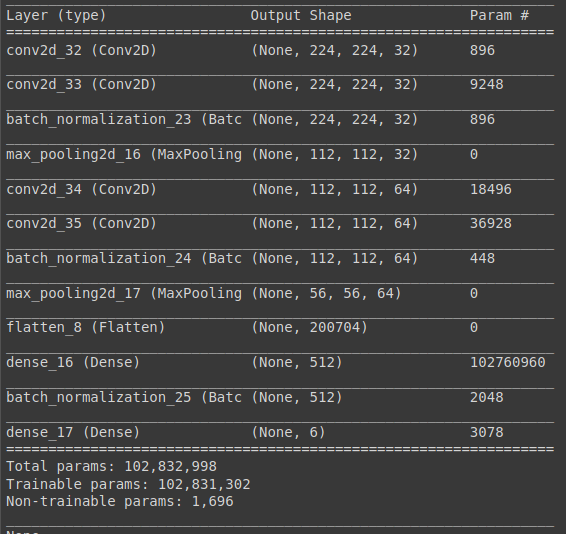
\includegraphics[width=0.8\textwidth]{images/q1/pd/q1pdmodel}
	\caption{Model Summary}
	\label{fig:q1pdmodel}
\end{figure}

The plots in Figures \ref{fig:q1pdacc} and \ref{fig:q1pdloss} show the
validation and training accuracies and losses respectively. The
validation accuracy shows that the model is not overfitting, and the loss is
relatively low.

\begin{figure}[H]
	\centering
	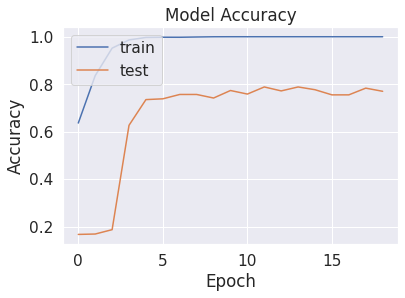
\includegraphics[width=0.8\textwidth]{images/q1/pd/accuracy}
	\caption{Validation and Training Accuracy}
	\label{fig:q1pdacc}
\end{figure}

\begin{figure}[H]
	\centering
	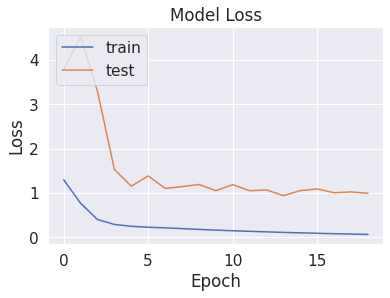
\includegraphics[width=0.8\textwidth]{images/q1/pd/loss}
	\caption{Validation and Training Loss}
	\label{fig:q1pdloss}
\end{figure}

The test output gives an average precision and recall of 80\%, with the highest
values attributed to the ``Parachute'' class, and the lowest values attributed
to the ``English Springer'' class.

\begin{figure}[H]
	\centering
	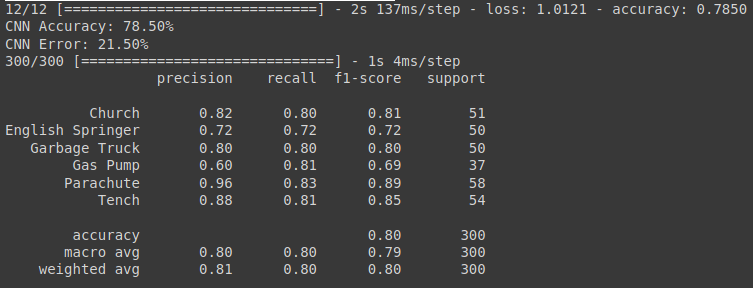
\includegraphics[width=0.8\textwidth]{images/q1/pd/q1pdresults}
	\caption{Model Testing Results}
	\label{fig:q1pdResults}
\end{figure}

The confusion matrix shows the number of correctly identified test samples, with
the highest precision class being ``Parachute'', labelled as ``4'' within the
matrix.

\begin{figure}[H]
	\centering
	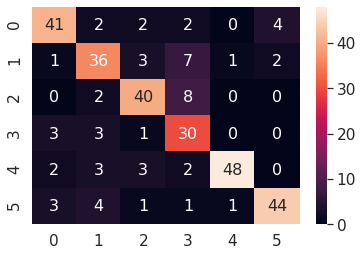
\includegraphics[width=0.8\textwidth]{images/q1/pd/matrix}
	\caption{Confusion Matrix}
	\label{fig:q1pdMatrix}
\end{figure}

Using early stopping, the model ran for a total of 19 epochs, The training time
for this model was 536.67 seconds, giving an emission output of 2.236lbs CO2
equivalent emissions. While this value is lower than Part c, it is higher than
that of Part a and Part b, showing the overhead involved with batch
normalisation.
